\chapter{Background}
\label{chap:background}

The subject of this work evolved from the situation, that the healthcare robotic applications of the University of Auckland should be equipped with mechanisms for ensuring safety.
The motivation for it is described in section~\ref{sec:healthbotapplication} as well as the robots, the kind of applications running on them, and their technical background.

The visual programming environment used for the programming of these robots is presented in section~\ref{sec:robostudio}.
For the understanding of safety concepts which this work is based on, a short introduction into the world of functional safety is given in section~\ref{sec:behaviourchecking}. In section~\ref{sec:relatedwork} other works and programs related to this work's topic are examined which also deal with safety aspects.




\section{Healhbot application}
\label{sec:healthbotapplication}

%\begin{wrapfigure}{r}{0.38\textwidth}
%  \centering
%  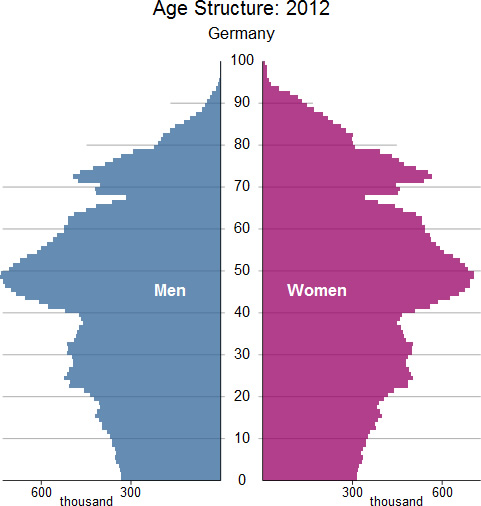
\includegraphics[width=0.34\textwidth]{populationpyramide}
%  \caption{Age structure.}%Population pyramide of germany.}
%  \label{fig:populationpyramide}
%\end{wrapfigure}
In some countries, among New Zealand and Germany, the average age of population is constantly increasing. Owing to excellent achievements in medicine as well as higher living standards, humans can enjoy longer lifes. Also decreasing birth rates contribute to an upward drift of the dominating age range. As a result, the industrial sectors of professional health care and social institutions are required more than ever.
However, a strong deficit of professionals is denoted in the healthcare branch and availability is far behind demand. One reason for this might be below average low salaries for employees in the healthcare sector. But, just raising the salary isn't leading to the desired results since the majority of the older people can't even afford a nurse to today's prices.

Aiming for fillig the constantly increasing gap in professional personnel for healtcare of the elderly and bypassing die financial burden, service robots are supposed to more and more undertake the task of care.
There are lots of possible tasks a robot could do such as taking the blood pressure, guiding medication intake, detecting falls or just entertaining with music, video or internet.
This challenge as a goal, the healtcare robotics team at the University of Auckland researches this topic and builds service robots for supporting the elderlies in their daily life.

The two newest robots IrobiQ and Cafero are shown in figure~\ref{fig:irobiq_cafero}.
These mobile 
\begin{wrapfigure}{r}{0.60\textwidth}
  \centering
  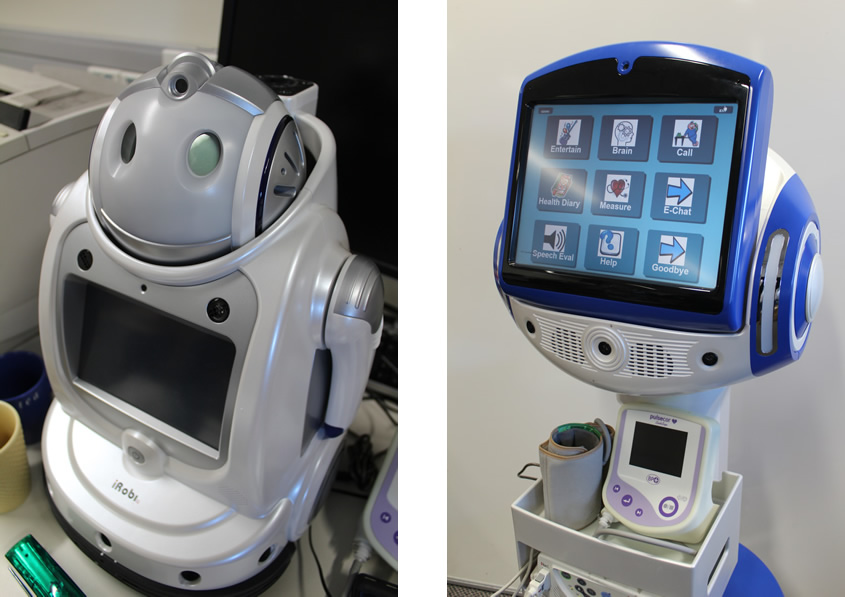
\includegraphics[width=0.56\textwidth]{irobiq_cafero}
  \caption{IrobiQ and Cafero, two robots of the healtcare project.}
  \label{fig:irobiq_cafero}
\end{wrapfigure}
robots have got a touch display for presenting screens and receiving user input. Furthermore they are equipped with additional external tools such as the blood pressure measurement device.
Applications running on the robot use the touch display to present screen dialogs to the user and use speech synthesis in order to give also accoustic feedbak. User inputs or response from devices cause dialogs to change. Figure~\ref{fig:screenflow_example} presents a little example of such a screen-flow based application, which uses response from a camera and user input for navigating through the screen-flow.

%, and they can access devices such as the camera for face recognition or the blood pressure measurement tool. 

There is a program interpreter running on the robots which can load and execute program files. Screen dialogs get generated and displayed on the touch screen.
%This makes the program behaviour replaceable and maintenance can be done easily.
The interpreter processes programs written in Robot Behaviour Description Language (RBDL), a particular DSL based on XML, which has been developed particularly for the healthcare robotic applications. It allows defining state machine based program behaviour and creating UI elements for screen visualizations. An example implementation of one state in RBDL is shown in listing~\ref{lst:RBDL}.

\begin{figure}[htbp]
  \centering
  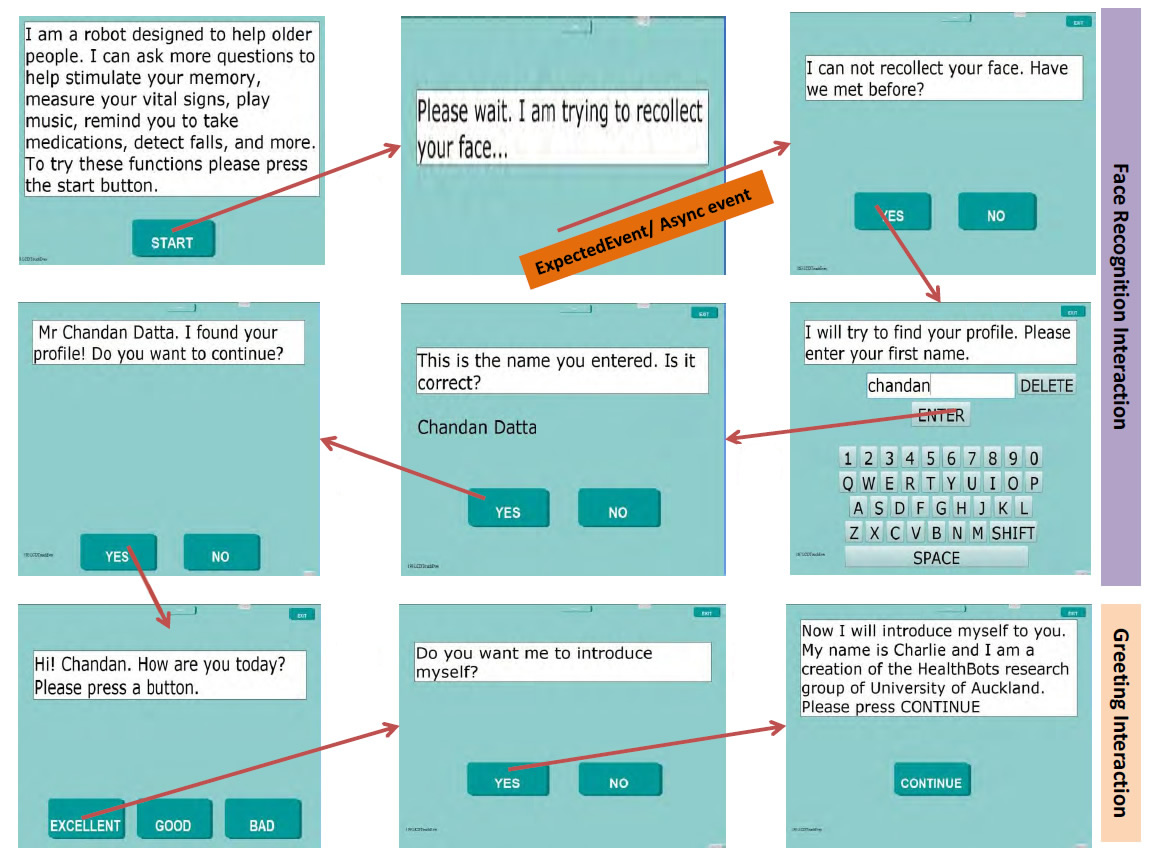
\includegraphics[width=\linewidth]{screenflow_example} 
  \caption{Robot screen-flow dialog based interaction example~\cite{robostudio}.}
  \label{fig:screenflow_example}
\end{figure}

\lstset{
  basicstyle=\ttfamily,
  columns=fullflexible,
  showstringspaces=false,
  commentstyle=\color{gray}\upshape
}

\lstdefinelanguage{XML}
{
  morestring=[b]",
  morestring=[s]{>}{<},
  morecomment=[s]{<?}{?>},
  stringstyle=\color{black},
  identifierstyle=\color{darkblue},
  keywordstyle=\color{cyan},
	morekeywords={%no, type_, senderid, receiverid, name_, vartype, label, width, height, x, y, textsize, preconditions
	}
}

\begin{lstlisting}[float = htbp, language=XML, captionpos=b, breaklines=true, showspaces=false, showtabs=false, tabsize=2, caption=Example of a state defined by RBDL~\cite{robostudio}., label=lst:RBDL]
<state no="84">
	<backgroundactions>
		<rocosmessage type="EVENT MESSAGE" senderid="RCP" receiverid="NA" name="FDSessionStart">
			<parameter vartype="text" type="unsigned int" name="id">1</parameter>
			<parameter type="string" name="" />
		</rocosmessage>
	</backgroundactions>
	<screen>
		<components>
			<button label="START" width="250" height="100" x="387" y="600" textsize="40">
				<event name="clicked">
					<action preconditions="no" name="transition">
						<parameter>
							<type>state</type>
							<name>n</name>
							<value>86</value>
						</parameter>
					</action>
				</event>
			</button>
		</components>
	</screen>
	<expectedevents>
		<event name="TimeOut">
			<action preconditions="no" name="transition">
				<parameter>
					<type>state</type>
					<name>n</name>
					<value>VARFirstScreen</value>
				</parameter>
			</action>
		</event>
	</expectedevents>
</state>
\end{lstlisting}

For each state of the program, backgroundactions can be defined. They are transparent to the user and run in background. Text messages can be sent or external devices can be acessed, for example. The latter is realized with web services to obtain a modular design.
Some states can also have screen definitions with buttons, messages, videos, etc. on it. These are displayed to the user when the particular state is active. Once displayed, buttons can be clicked and trigger events.
The behaviour of events can be mapped in the expectedevents tag. It lists all events which are processable by the current state and defines the correspondend behaviour such as triggering transitions to other states.

For this work the most important thing about the RBDL to remember is, that it can define state machine behaviour with states, transitions and events. This fact was basement for later decisions regarding used safety mechanisms.



%Zugriff auf devices via web services
%Windows is used as operating system on the robots and the programs are executed in Adobe flash and Actionscript. External devices are accessed over web




\section{Robostudio}
\label{sec:robostudio}

In the beginning all programming of the robot behaviour was done by directly editing the XML code mentioned in the previous section by using a text editor. But huge code files and occasional code edits made further maintenance and change requests difficult up to impossible to realise. For this reason Chandan Datta, PhD student at the University of Auckland, developed a visual programming environment for developing robot behaviour on top of RBDL: Robostudio~\cite{robostudio} allows to easily edit the program behaviour on a visual layer and generates the corresponding program file containing the RBDL code fully automatically. This file can be downloaded to the robot and executed by the interpreter. Figure~\ref{fig:robostudio_proceeding} illustrates what the steps of robot behaviour development are.

\begin{figure}[htbp]
  \centering
  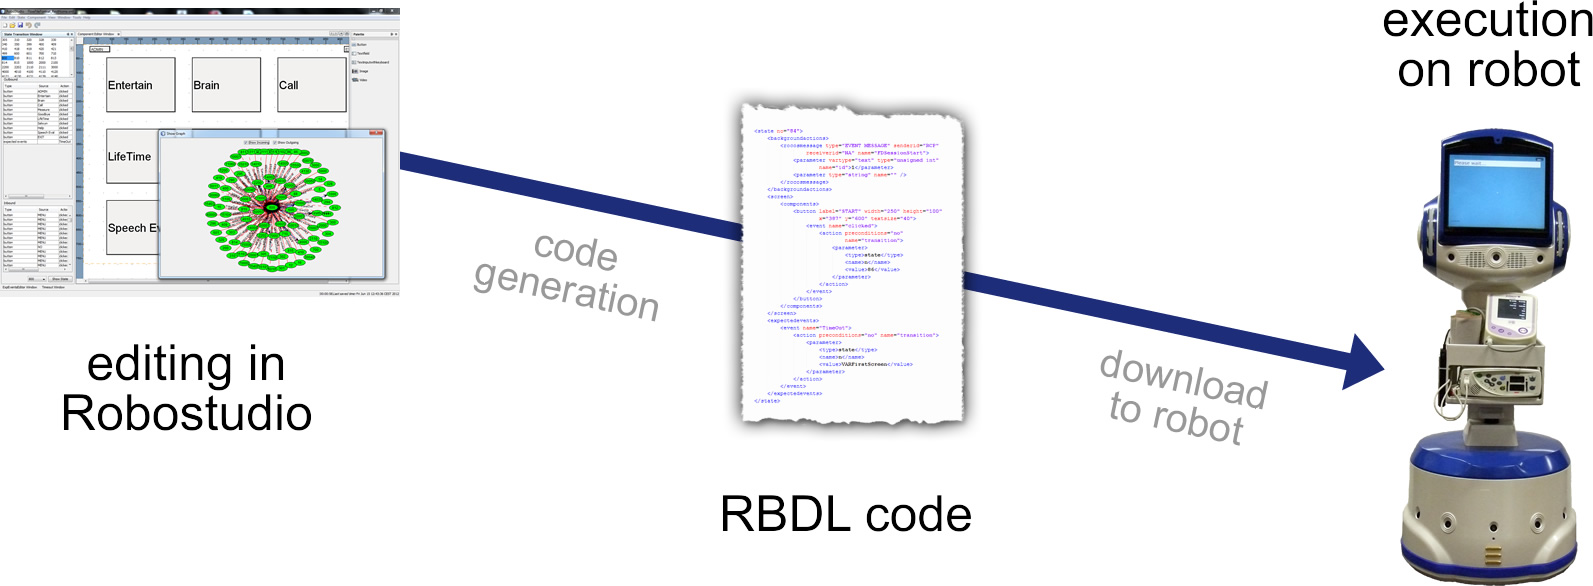
\includegraphics[width=\linewidth]{robostudio_proceeding} 
  \caption{How Robostudio is used for robot behaviour development.}
  \label{fig:robostudio_proceeding}
\end{figure}

Robostudio is an editor fully written in Java and implemented as a NetBeans rich client application.
In several windows and views there are visual tools for editing and understanding robot behaviour as well as screen dialog design. As depicted in figure~\ref{fig:robostudio_vpe} the editor has got a State Navigator Window (1) in the top left corner where all existing states are listed. Underneath an overview about all incoming and outgoing transitions is given. New states can be created and existing states can be deleted. A click on one particular state id in the State Navigator Window will cause all other components to show all possible information regarding to the selected state.
The Expected Events Editor Window (2) in the bottom left provides specifying the expected events and their effects.
Heart and center of the editor is the UI Component Layout Editor Window (3). It renders the screen dialog of the selected state and gives a preview of the screen presented on the robot during runtime. Components such as buttons, text boxes or images can be added, changed or removed via drag and drop.
They are provided by the UI Components Palette Window (4) on the right side where the user can choose from all supported UI components.
The Background Actions Editor Window (5) lets the user define background actions, which are executed trasparently to the user such as accessing external devices or sending messages.
Aiming for supporting the developer with helpful graphical tools the State Transition Visualization Window (6) gives an overview about all connections towards and from the selected state. It helps to quickly get an understanding of the local program behaviour.

\begin{figure}[htbp]
  \centering
  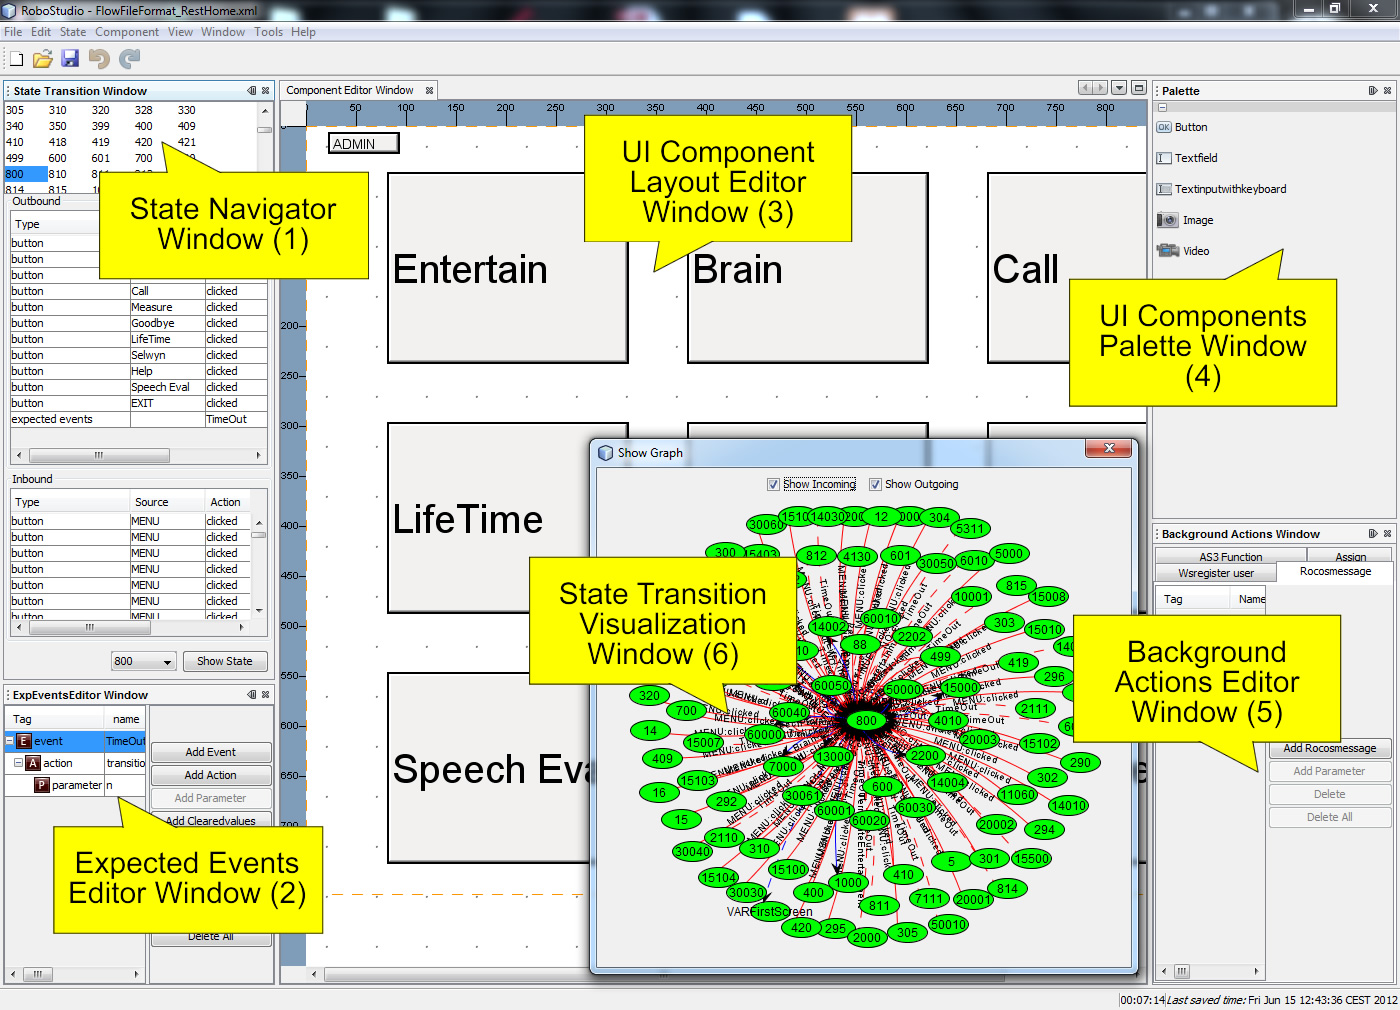
\includegraphics[width=\linewidth]{robostudio_vpe} 
  \caption{Window composition in Robostudio.}
  \label{fig:robostudio_vpe}
\end{figure}


%TODO: Vlt herausstellen, dass eine Schwierigkeit darin bestand, Verhaltensmodellierung und graphische Gestaltung unter einen Hut zu bringen (dazu Bild aus datta paper?). One challenge...






\section{Behaviour checking}
\label{sec:behaviourchecking}

The use of software is versatile from text editing programs running on personal computers, over control software for high-precision applications in aeronautics, right up to trigger mechanisms for deathly weapons. For most of them safety properties are irrelevant, but a few are ranked highly dangerous to their environment and also human lifes. In order to eliminate software malfunction there are a lot of mathematical concepts for verifying software behaviour.
One of them is model checking wich allows checking for functional safety on state machine programs. Since we deal with state machines in the healthbot applications mentioned in section~\ref{sec:healthbotapplication}, this concept of behaviour checking is applicable and important for our kind of programs. At first the basic idea of state machines is described in section~\ref{sec:statemachines}, followed by an intorduction into model checking in section~\ref{sec:modelcheckingandltl}.


\subsection{State machines}
\label{sec:statemachines}



\subsection{Model checking \& LTL}
\label{sec:modelcheckingandltl}

%CTL and LTL are important concepts for model checking and verification of statemachines. But their powerfulness is reflected in the complexity of their mathematical expressions, what makes it difficult to use for programmers who haven't got deeper expertise in this subject.


%NuSMV erwaehnen, erklaeren warum nicht CTL? ltl passt fuer healthcare besser






\section{Related work}
\label{sec:relatedwork}


%Was gibt es schon alles?

% 1993 A Visual-Programming Environment for a Temporal Logic Language
% 1995 Visual Specification of Branching Time Temporal Logic
% 2007 HomeTL: A visual formalism, based on temporal logic, for the design of home based care
% 2007 A Visual Editor to Support the Use of Temporal Logic for ADL Monitoring


A first step towards a graphical tool for designing safety constraints is taken by Sisiruca and Ionescu~\cite{332301}. They developed an object-oriented graphical environment for visually creating temporal logic sentences and rules. The tool presents temporal operators as logical modules with boolean inputs and outputs which can be connected to one big expression graph. Del Bimbo et al. worked on a visual tool for temporal logic, but with a special focus on hierarchical representation of formulas~\cite{520786}. Here each node of a tree is described by an abstract operator whose subformulas are branches to their replacement operators. Thus the root node represents the entire formula. They also explored the formula trees' 3D representation within a virtual space. Both approaches are different fundamental ideas of representing temporal formulas. Whereas having a graph  seems not to be applicable for our approach, the idea of hirarchical operator representation of Del Bimbo et al. will be a good basis for our concept of constraint creation and understanding.

%aim for simplifying the development of constraints, but they still demand knowledge of the underlying mathematical formalism of temporal logic.

The step towards a more abstract level of development is taken by HomeTL~\cite{4341725}, a visual formalism for the design of home based care. It allows healthcare professionals to specify rules and sequences of user actions in a quite nontechnical manner. Based on these conditions a monitoring system in a patient's home environment can detect and report abnormal situations within the daily routine. Even though this approach touches the subject of healthcare it barely matches our problem. HomeTL focuses more on monitoring temporal boundaries of a patient's behaviour than on ensuring functional safety of an implemented program. It does depict how nontechnical constraint design can be realised and its graphical design is a good example of handling time dependencies.

%There are already works about constraint generation such as one approach of NASA [4], for example. They used test oracles in order to achieve consistency between program code and specification during development. 
% Das wollen wir auch erzielen mit unseren automatisch generierten constraints...

%But these kind of oracles are for automated test purpose and are rather complex than intuitive. However, our goal is to find nonmathematical and just intuitive ones. An intelligent heuristic must determine key states and possible conjunctions of them in order to build reasonable constraints. Afterwards they get filtered by an algorithm which computes importances for each constraint based on state weights. Finally the developer obtains a set of visual constraints which he can then check for plausibility.





\subsection{Sisiruca and Ionescu}
\subsection{Del Bimbo (3D)}
\subsection{HomeTL}